% !TEX root = ../report.tex
\chapter{Analysis}
\label{ch:analysis}

%All layers (with their patterns) is very clearly described in ch8 starting on p95.

\newcommand{\EAA}{Patterns of Enterprise Application Architecture}

%\section{Layers}
%
%\begin{description}
%%
%%Context – a recurring set of situations in which the
%%pattern applies.
%%Problem - a set of forces (goals and constraints)
%%occurring in this context.
%%• Forces are often competing
%%Solution - a canonical design form or rule that
%%someone can apply to resolve these forces.
%%• The solution balances the forces.
%
%\item [Context]
%
%
%\item [Problem]
%The system needs a structure to coordinate the external calls and requests.
%
%\item [Solution]
%Our application exposes a web service to multiple clients and so a the Service Layer pattern will be used. Using this pattern, the system will be divided into the following layers.
%
%
%
%\item [Source] 
%\EAA  \cite{Fowler:2002:PEA:579257}
%\end{description}

\section{Layers}
\manuallabel{sec:layers}{Layers}

\begin{description}
\item [Source]~\\
Pattern-oriented Software Architecture - Volume 1 \cite{wiley-1}

\item [Issue]~\\
The system consists of high-level components (e.g. user interface), which are dependent on lower level components (domain logic, database). Decoupling these components is important.

\item [Assumptions/Constraints]~
\begin{itemize}
\item It is assumed that the system will have higher-level components that depend on lower-level components.
\end{itemize}
~\\[-1.5cm]

\item [Positions]~
\begin{enumerate}
\item Relaxed Layered System
\item Layers
% Indirection Layers??
\end{enumerate}
~\\[-1.5cm]

\item [Decision] ~\\
The system will use the Layers pattern to divide the application in multiple layers. The top layer will implement the Service Layer pattern, the middle layer will implement the domain logic (domain model) and the bottom layer will be responsible for the data storage.

\item [Argument]~
\begin{enumerate}
\item The relaxed layered system is a variant of the Layers pattern which allows layers to use services of any layer below it, instead of only the next layer. This increases the flexibility and performance of the system. However, this pattern has a large negative impact on the maintainability.

\item 
Using the layers pattern increases maintainability by decoupling components of different levels of abstraction.

\end{enumerate}

\item [Implications]~\\
Using layers will have a positive impact on the maintainability and re-usability of the system. An increased maintainability will help prevent bugs, which on the longer term helps to increase the reliability of the system. 

The performance of the system will have some negative impact, since the request have to pass all the layers, even if they only need logic/data in the bottom layer.

\item [Related requirements/decisions]~\\
\ref{sec:service-layer}, 

\end{description}


\section{Service Layer}
\manuallabel{sec:service-layer}{Service Layer}

\begin{description}
\item [Source]~\\
Patterns of Enterprise Application Architecture, P.133 \cite{Fowler:2002:PEA:579257}

\item [Issue]~\\
The system will have different interfaces with different kinds of clients. For example, commands to compute statistics can come from the user interface, but also from the alerting module. These different interfaces have common interactions with the system to invoke the business logic. %TODO describe altering module in elaborated model

\item [Assumptions/Constraints]~
\begin{itemize}
\item The application's business logic and/or data are accessed using several interfaces.
\end{itemize}

\item [Positions]~
\begin{enumerate}
\item Domain Model % just domain model not good enough
\item Service Layer
\end{enumerate}
~\\[-1.5cm]

\item [Decision] ~\\
The system will use the Service Layer pattern to define the boundary of the application using a layer of services.

The service layer exposes a set of services to be used by clients and for each service, there is a certain script that will be executed when the service is called. The service layer will be used with the "operation script" variation. This means that the Service Layer consists of thick classes that contain logic. %TODO Why do we want thick classes with logic?????

\item [Argument]~
\begin{enumerate}
\item Using just the Domain Model pattern alone does not make a distinction between application logic and domain logic.

\item The service layer does allow making a distinction between the application- and domain logic, which 
\end{enumerate}

\item [Implications]~\\
There is a boundary between the application- and domain logic.

\item [Related requirements/decisions]~\\
\ref{sec:layers}, \ref{fr:interface-selectstats}, \ref{fr:receive-usage}

\begin{figure}[H]
\caption{Service Layer}
\centering
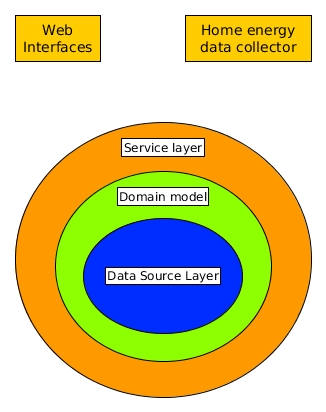
\includegraphics[scale=0.7]{4-analysis/images/ServiceLayer.jpg}
\end{figure}


\end{description}


%\section{Layer Supertype}
%
%\begin{description}
%%
%%Context – a recurring set of situations in which the
%%pattern applies.
%%Problem - a set of forces (goals and constraints)
%%occurring in this context.
%%• Forces are often competing
%%Solution - a canonical design form or rule that
%%someone can apply to resolve these forces.
%%• The solution balances the forces.
%
%%\begin{description}
%%\item [Context]
%%\item [Problem]
%%\item [Solution]
%%\item [Source]
%
%\item [Context]
%There is duplicate code within each layer of the system.
%
%\item [Problem]
%Duplicate code makes the system hard to modify and maintain.
%
%\item [Solution]
%With the Layer Supertype pattern, all the classes of a certain layer have the same super class. This super class then contains the features that are very common for the layer.
%
%This pattern will be used in every layer.
%\begin{description}
%\item[Service layer] All the services need to take care of security. The client needs to be authenticated and the data needs to be decryption by the service layer. All this security logic will be placed in a super type using the "Layer Supertype" pattern In the service layer it contains the security logic.
%
%\item[Domain layer] In this layer, the sypertype will contain common features and functions for handling storage.
%%\myworries{From book:
%%-  "Common features, such as the storage and handling of 'Identity Fields (216), can go there."}
%
%\item[Data source layer]
%The data mapper in the data source pattern can use a layer super type that handles all the common behavior, which can greatly reduce the extra work of coding. 
%
%%(p308 (Metadata mapping pattern))
%\end{description}
%
%%\myworries{p475 POEAA
%%"A type that acts as the super type for all types in the layer".}
%
%\end{description}

\section{Domain layer}

\begin{description}
\item [Context]
The domain logic consists of complex functions for serving web request and analyzing data.

\item [Problem]
The functionality of the system must be modifiable and must not contain duplicate code to prevent inconsistency.

\item [Solution]
The domain logic is complex and so it requires the use of the domain model pattern. This means that the domain is Object Oriented, with every class representing one specific, individual, meaningful part.
This is the most advanced pattern, reducing code duplication and increasing flexibility of the system.

%The alternatives are : Transaction Script and Table module.
%
%Transaction script: Each system call has its corresponding script that will be executed.\\
%Table module: One class per table in the database that contains all the logic acting on that data.

\item [Source]

\end{description}

\section{Unit of work}

\begin{description}
\item [Source]~\\
Patterns of Enterprise Application Architecture, P.184 \cite{Fowler:2002:PEA:579257}

\item [Issue]~\\
The system has several object stored in a database which can be edited and created. For example, new sensor data of devices becomes available and changes to the configuration (changing device names etc.) can be made. Updating database records on each change leads to a lot of database calls, which is bad for performance.

\item [Assumptions/Constraints]~\\

\item [Positions]
\begin{enumerate}
\item Active Record
\end{enumerate}

\item [Decision] ~\\
Unit of Work pattern will be used to keep track of changes to objects and to coordinate writing these changes to the database in one database call.

\item [Argument]~\\
With Active Record, every change to an in-memory object leads to a database call. This means that multiple consecutive changes to an object lead to multiple database calls. 

The Unit of Work instead keeps track of these changes, to allow writing these changes to the database in a single call.

\item [Implications]~\\
Using Unit of Work will reduce the load on the database (the number of database calls). It does however introduce a delay before the change in the in-memory object is present in the representation in the database.

\item [Related requirements/decisions]~\\
--

\end{description}

\section{Broker}

\begin{description}
\item [Source]~\\
Pattern-oriented Software Architecture - Volume 4 \cite{wiley-4}

\item [Issue]~\\
The system uses several servers to compute the statistics. This introduces a lot of challenges, like communication to these servers and dividing the work over these servers. The application code should not have to address these challenges.

\item [Assumptions/Constraints]~\\

\item [Positions]~
\begin{enumerate}
\item Publisher-Subscriber
\item Broker
\item Message Queuing
\item Remote Procedure Call
\end{enumerate}
~\\[-1.5cm]

\item [Decision] ~\\


\item [Argument]~\\


\item [Implications]~\\


\item [Related requirements/decisions]~\\
\ref{fr:compute-total}, \ref{fr:compute-bill}, \ref{fr:compute-bill}
%Refer to layers
%Most B ROKER realizations are based on a L AYERS (185) architecture
%to manage complexity, such as CORBA [OMG04a] and Microsoft’s
%.NET Remoting [Ram02]. These layers are further decomposed into
%‘special-purpose’ components for specific networking and communi-
%cation tasks. We illustrate this partitioning using the CORBA layering
%[SC99]—other layering schemes and middleware may involve differ-
%ent assignments [VKZ04].

\end{description}


\section{Data source layer}
The main database will be quite simple and the database actions won't be very complicated. However, the tables needed for the statistics can become very complex.

\begin{figure}[H]
\caption{Database structure draft}
\centering
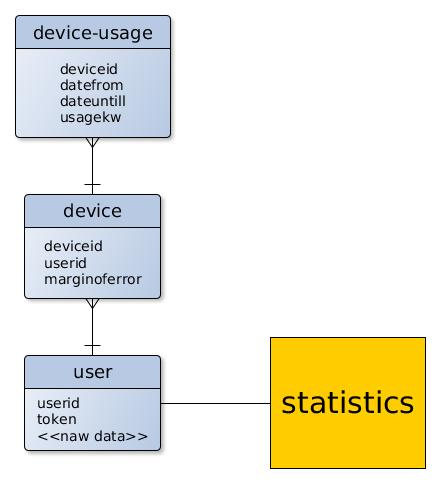
\includegraphics[height=10cm]{4-analysis/images/SoftwarePatternsDatabaseDraft.jpg}
\end{figure}

Considered patterns to connect to data sources:
\begin{itemize}
\item Table data gateway% (p144)
\item Row data gateway% (p152)
\item Active record %(p160)
\item Data mapper% (p165)
\end{itemize}

Because the domain model is used in the domain layer, the data mapper pattern is best to use . \ign{(153 and 97)}
The logic that will operate on the data will generate statistics of the data, which can become quite complex. This is why the data mapper pattern is chosen as a pattern for connecting to the data sources. This pattern is the most advanced pattern, but provides the best functionality and abstraction.

With the active record pattern, the database access/communication, data and logic of that data is all stored in the same class. Since the logic that will be executed on the sensor data is very complex, this patterns will not be useful.

A gateway of any kind leads to performance overhead, because for each call coming from the domain model pattern, a database call is made. It lacks the necessary coordination.
%
%\subsection{Table data gateway}
%\myworries{Not needed if the repository is used (i assume)}
%
%The data mapper can use the table data gateway to remove the dependency on how the data is queried. Queries can be replaced with stored procedures in the Table data gateway without the data mappers having to change 
%
%%Using a record set (504) turning into a unit of work (184)? P98 (lost the page:()

\subsection{Repository}
%\myworries{
%P322:
%"Mediates between the domain and data mapping layers using a collection-like interface for accesing domain objects."
%\\
%P323:
%"Repository supports the objective of achieving a clean separation and one-way dependency between the domain and data mapping layers"
%\\
%P324:
%"Under the covers, Repository combines Metadata Mapping (329) with a Query object (316) to automatically generate SQL code from the criteria."
%...
%"In a large system with many domain object types and many possible queries, Repository reduces the amount of code needed to deal with all the querying that go's on."
%}

The repository pattern mediates between the domain and data layer. The repository clients create a criteria object, specifying what kind of data is wanted. For example $criteria.equals(Device.NAME, Computer)$. Then the clients use this criteria by invoking repository.matching(criteria) to receive the data from the repository. The client just asks the data, it has no further knowledge about any interaction with any data source/data base.

The repository gives a lot more control over how the data is handled. The benefits are:
\begin{itemize}
\item Reduces code (and code complexity)
\item Increases performance
\item Separated domain and data layers, increasing flexibility and changeability
\end{itemize}

Performing analysis on the data also consists of executing complex queries on the data source. The database that executes these queries, however, might change. Or the system might decide to use multiple databases and data sources.
Using the Repository pattern, these changes can be made fast. The repository also allows for multiple configurations to exist. So an extra repository could be created for testing purposes, only using an in-memory database to increase the test execution speed.

\section{Client user interface}

\subsection{Controller}
%\myworries{
%On p 99:
%\begin{itemize}
%\item Given a free choice, I'd recommend Page Controller (p333). 
%\item More complex navigation and UI lead you toward a Front Controller (344)
%\end{itemize}
%}
Page controller: controller for each page. So upon receiving a request do:
\begin{itemize}
\item decode url, extract data
\item invoke model to process data
\item determine view and use the model data to create the HTML to return
\end{itemize}

Front page controller:\\
One controller for all requests/views. This allows building a filter chain, handling authentication, logging etc.
Front page is better/helps with concurrency, because a new command object is created on each request. Reducing thread-safety concerns. \ign{(P346)}The model, however, can have shared objects that do require thread safety management.

The front page will be used, because it provides more functionality to the system. The only advantage of a page controller compared to the front controller is that it has a more natural structure.

\subsection{View}
%\myworries{
%Template view (350) or Transform view (361).
%\\
%(P forgot):
%Template views have the edge at the moment.
%}

\begin{description}
\item [Template view] Write HTML code including markers. Replace the markers with the data when the page is requested. (Play framework)
\item [Transform view] Convert the domain data to HTML, "transform" the domain data. Upon a request, it get the domain data, for each item in the data it looks for a appropriate "transform" to transform the data to HTML.
\end{description}

The template view will be used, because it is used a lot more then the transform view. Major web frameworks are based on this pattern (the play framework, laravel...). The view patterns don't have an important difference in how beneficial they are to the project.

%Transform view avoids having too much data in the HTML, because of the transform methods creating the HTML.
%Transform view can be tested without having a web server up.

\subsection{Model}
%\myworries{
%Communication with the model: p100:
%Preference: Having everything run in one process if you can. Else Remote Facade (p388) and DTO (p 401).
%}
%
%\myworries{
%\section{Notes only}
%\subsection{Model-View View-Model}
%}
This section will describe how the Model updates the view and how the view updates the model.
%\myworries{View update model using page controller as is already described}

To consider:
\begin{description}
\item [Observer Synchronization] Synchronize multiple screens by having them all be observers to a shared area of domain data.
\item [Separated Presentation] Ensure that any code that manipulates presentation only manipulates presentation, pushing all domain and data source logic into clearly separated areas of the program.

\item [Presentation model] Represent the state and behavior of the presentation independently of the GUI controls used in the interface

\item [Supervising controller] Factor the UI into a view and controller where the view handles simple mapping to the underlying model and the the controller handles input response and complex view logic.

\item [Model view controller/presenter] 

\end{description}

%Observer Synchronization
%%Synchronize multiple screens by having them all be observers to a shared area of domain data.
%%\url{http://www.martinfowler.com/eaaDev/uiArchs.html}
%%While Observer Synchronization is nice it does have a downside. The problem with Observer Synchronization is the core problem of the observer pattern itself - you can't tell what is happening by reading the code. I was reminded of this very forcefully when trying to figure out how some Smalltalk 80 screens worked. I could get so far by reading the code, but once the observer mechanism kicked in the only way I could see what was going on was via a debugger and trace statements. Observer behavior is hard to understand and debug because it's implicit behavior.
%
%Separated Presentation:
%%\url{http://martinfowler.com/eaaDev/SeparatedPresentation.html}
%Ensure that any code that manipulates presentation only manipulates presentation, pushing all domain and data source logic into clearly separated areas of the program.
%%Most of examples you'll see from me follow Separated Presentation, simply because I find it such a fundamental design technique
%
%Presentation model:
%%\url{http://www.martinfowler.com/eaaDev/PresentationModel.html}
%Represent the state and behavior of the presentation independently of the GUI controls used in the interface
%
%Supervising controller\\
%Factor the UI into a view and controller where the view handles simple mapping to the underlying model and the the controller handles input response and complex view logic.
%
%%MVP potel:
%%\url{Potel: http://www.wildcrest.com/Potel/Portfolio/mvp.pdf}
